\documentclass[letterpaper]{article}
\usepackage{typearea}
\typearea{12}
\usepackage{here}
\usepackage{bm}
\usepackage{amsmath, amsfonts}
\usepackage[top=20truemm,bottom=20truemm,left=25truemm,right=25truemm]{geometry}
\usepackage[dvipdfmx]{hyperref,graphicx}
\usepackage{xeCJK}

% incorporated from Linear Algebra for Everyone 7/18/2022
\newcommand{\bi}[1]{\hbox{\boldmath$#1$}}
\DeclareRobustCommand\transp{^{\mathrm{T}}}
\DeclareMathAlphabet{\cmrv}{OML}{cmm}{b}{it}
\newcommand{\bu}{\hbox{\boldmath$u$}}
\newcommand{\bv}{\hbox{$\cmrv{v}$}}
\newcommand{\bw}{\hbox{\boldmath$w$}}
\newcommand\mat{{\sf MATLAB}}
%

% prepare to move figures
\graphicspath{ {figs/} }

\begin{document}
\title{The Art of Linear Algebra\\
\vspace{5pt}
\large{
-- Graphic Notes on ``Linear Algebra for Everyone" --
}
}

\author{Kenji Hiranabe
\thanks{twitter: @hiranabe, k-hiranabe@esm.co.jp, \url{https://anagileway.com}} \\
with the kindest help of Gilbert Strang
\thanks{Massachusetts Institute of Technology, \url{http://www-math.mit.edu/\~gs/}} \\
translator: Kefang Liu
\thanks{twitter: \href{https://twitter.com/KFChLiu}{@kfchliu}, 微博用户: \href{https://weibo.com/u/5717297833}{5717297833}}
}

\date{September 1, 2021/updated \today}

\maketitle

\vspace{-5pt}
 
\begin{abstract}
我尝试为 Gilbert Strang 在书籍 “Linear Algebra for Everyone” 中介绍的矩阵的重要概念进行可视化图释, 
以促进从矩阵分解的角度对向量、矩阵计算和算法的理解.
\footnote{``Linear Algebra for Everyone": 
\url{http://math.mit.edu/everyone/}.}
它们包括矩阵分解 (Column-Row, $\bm{CR}$)、
高斯消去法 (Gaussian Elimination, $\bm{LU}$)、
格拉姆-施密特正交化 (Gram-Schmidt Orthogonalization, $\bm{QR}$)、
特征值和对角化 (Eigenvalues and Diagonalization, $\bm{Q \Lambda Q\transp}$)、
和奇异值分解 (Singular Value Decomposition, $\bm{U \Sigma V\transp}$).
\end{abstract}

\section*{序言}
我很高兴能看到 Kenji Hiranabe 的线性代数中的矩阵运算的图片! 
这样的图片是展示代数的绝佳方式. 我们当然可以通过 行 $\bm{\cdot}$ 列 的点乘来想象矩阵乘法, 
但那绝非全部 —— 它是``线性组合"与``秩1矩阵"组成的代数与艺术. 
我很感激能看到日文翻译的书籍和 Kenji 的图片中的想法. 
\begin{flushright}
-- Gilbert Strang \\ 麻省理工学院数学教授
\end{flushright}

\tableofcontents

\section{理解矩阵——4个视角}

一个矩阵 ($m \times n$) 可以被视为$1$个矩阵, $mn$个数, $n$个列和$m$个行.

\begin{figure}[H]
  \centering
  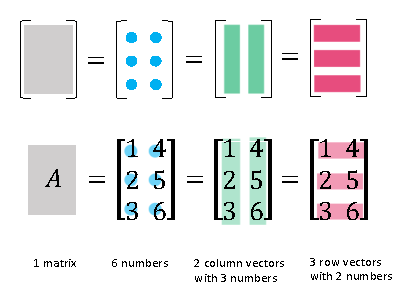
\includegraphics[scale=0.8]{ViewingMatrix-4Ways.eps}\\
    \caption{从四个角度理解矩阵}
\end{figure}


\begin{equation*}
  A= \begin{bmatrix}
    a_{11} & a_{12}\\
    a_{21} & a_{22}\\
    a_{31} & a_{32}
  \end{bmatrix}
  =
  \begin{bmatrix}
    | & |\\
    \bm{a_1} & \bm{a_2}\\
    | & |
  \end{bmatrix}
  =
  \begin{bmatrix}
    - \bm{a_1^*} -\\
    - \bm{a_2^*} -\\
    - \bm{a_3^*} -
  \end{bmatrix}
\end{equation*} \\

在这里, 列向量被标记为粗体$\bm{a_1}$.
行向量则有一个$\bm{*}$号, 标记为$\bm{a_1^*}$.
转置向量和矩阵则用$\mathrm{T}$标记为
$\bm{a}\transp$和$A\transp$.

\section{向量乘以向量——2个视角}

后文中, 我将介绍一些概念, 同时列出“Linear Algebra for Everyone”一书中的相应部分 (部分编号插入如下). 
详细的内容最好看书, 这里我也添加了一个简短的解释, 以便您可以通过这篇文章尽可能多地理解. 
此外, 每个图都有一个简短的名称, 例如 v1 (数字 1 表示向量的乘积)、Mv1 (数字 1 表示矩阵和向量的乘积), 以及如下图 (v1) 所示的彩色圆圈. 
如你所见, 随着讨论的进行, 该名称将被交叉引用. 

\begin{itemize}
  \item 1.1节 (p.2) Linear combination and dot products
  \item 1.3节 (p.25) Matrix of Rank One
  \item 1.4节 (p.29) Row way and column way
\end{itemize}

\begin{figure}[H]
  \centering
  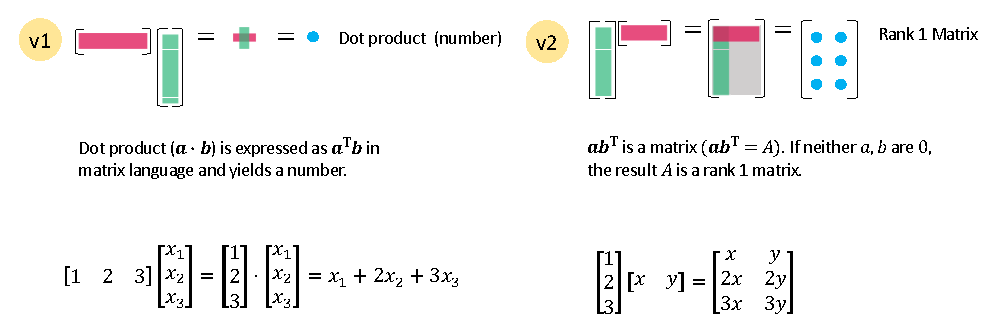
\includegraphics[scale=0.8]{VectorTimesVector.eps}
  \caption{向量乘以向量 - (v1), (v2)}
\end{figure}

(v1) 是两个向量之间的基础运算, 而 (v2) 将列乘以行并产生一个秩1矩阵. 
理解 (v2) 的结果 (秩1) 是接下来章节的关键.

\section{矩阵乘以向量——2个视角}

一个矩阵乘以一个向量将产生三个点积组成的向量 (Mv1) 和
一种$A$的列向量的线性组合.

\begin{itemize}
  \item 1.1节 (p.3) LInear combinations
  \item 1.3节 (p.21) Matrices and Column Spaces
\end{itemize} 

\begin{figure}[H]
  \centering
  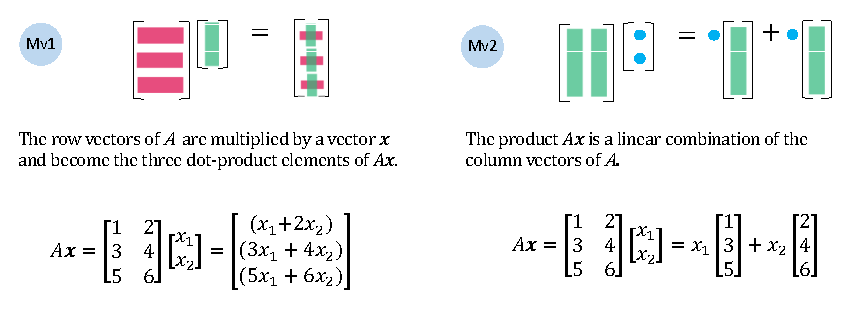
\includegraphics[scale=0.8]{MatrixTimesVector.eps}
  \caption{矩阵乘以向量- (Mv1), (Mv2)}
\end{figure}

往往你会先学习 (Mv1). 但当你习惯了从 (Mv2) 的视角看待它, 会理解$A\bm{x}$是$A$的列的线性组合. 
矩阵$A$的列向量的所有线性组合生成的子空间记为$\mathbf{C}(A)$. 
$A\bm{x}=\bm{0}$的解空间则是零空间, 记为$\mathbf{N}(A)$. 


同理, 由 (vM1) 和 (vM2) 可见, 行向量乘以矩阵也是同一种理解方式. 

\begin{figure}[H]
  \centering
  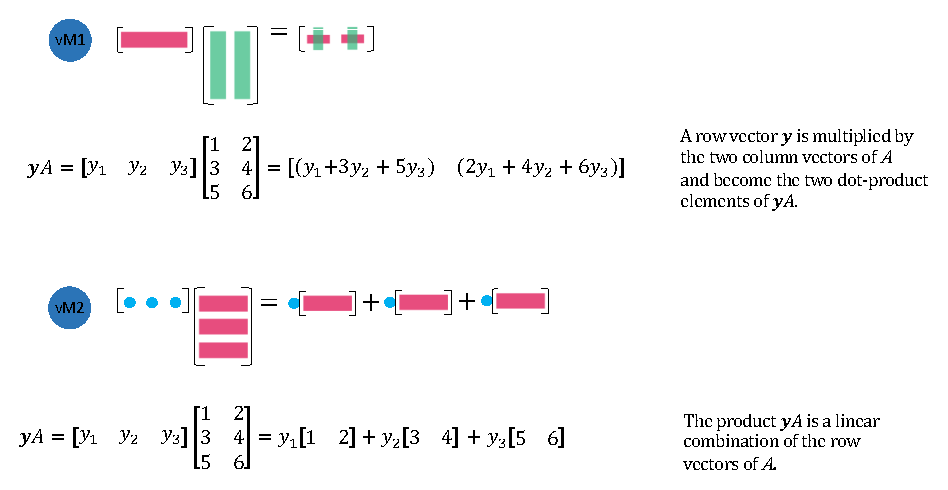
\includegraphics[scale=0.8]{VectorTimesMatrix.eps}
  \caption{向量乘以矩阵 - (vM1), (vM2)}
\end{figure}

上图$A$的行向量的所有线性组合生成的子空间记为$\mathbf{C}(A\transp)$. 
$yA=0$的解空间是$A$的左零空间, 记为 $\mathbf{N}(A\transp)$. 


本书的一大亮点即为四个基本子空间: 在$\mathbb{R}^n$ 上的
$\mathbf{N}(A)$ + $\mathbf{C}(A\transp)$ (相互正交) 
和在$\mathbb{R}^m$ 上的$\mathbf{N}(A\transp)$ + $\mathbf{C}(A)$ (相互正交). 


\begin{itemize}
  \item 3.5节 (p.124) Dimensions of the Four Subspaces
\end{itemize} 

\begin{figure}[H]
  \centering
  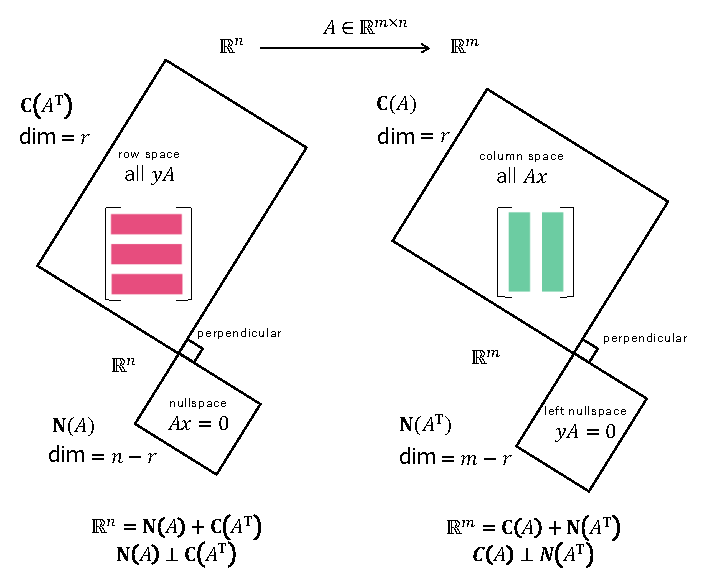
\includegraphics[keepaspectratio, width=8cm]{4-Subspaces.eps}
  \caption{四个子空间}
\end{figure}

关于秩$r$, 请见$A=CR$ (6.1节) .


\section{矩阵乘以矩阵——4个视角}

由``矩阵乘以向量"自然延伸到``矩阵乘以矩阵".

\begin{itemize}
  \item 1.4节 (p.35) Four ways to multiply $\bm{AB=C}$
  \item 也可以见书的封底
\end{itemize} 


\begin{figure}[H]
  \centering
  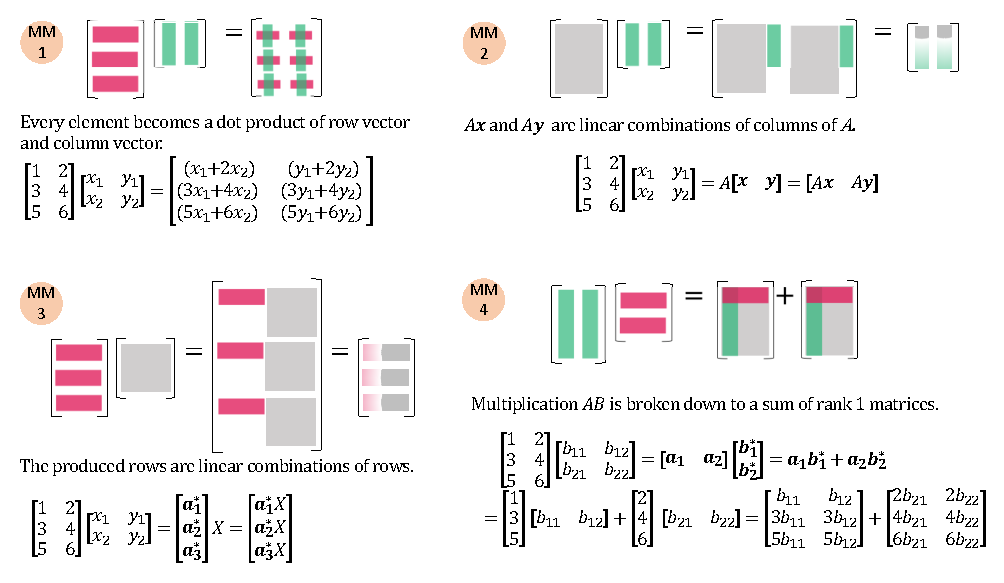
\includegraphics[scale=0.8]{MatrixTimesMatrix.eps}
  \caption{矩阵乘以矩阵 - (MM1), (MM2), (MM3), (MM4)}
\end{figure}

\section{实用模式}

在这里, 我展示了一些实用的模式, 可以让你更直观地理解接下来的内容。

\begin{figure}[H]
  \centering
  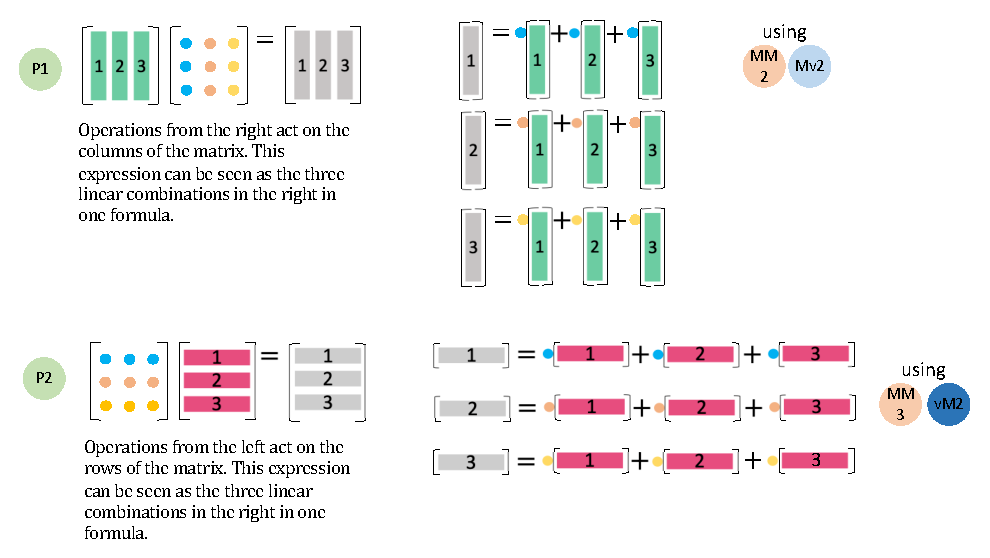
\includegraphics[scale=0.8]{Pattern12.eps}
  \caption{图 1, 2 - (P1), (P1)}
\end{figure}

P1 是 (MM2) 和 (Mv2) 的结合. 
P2 是 (MM3) 和 (vM2) 的扩展. 
注意, P1 是列运算 (右乘一个矩阵), 
而 P2 是行运算 (左乘一个矩阵). 

\begin{figure}[H]
  \centering
  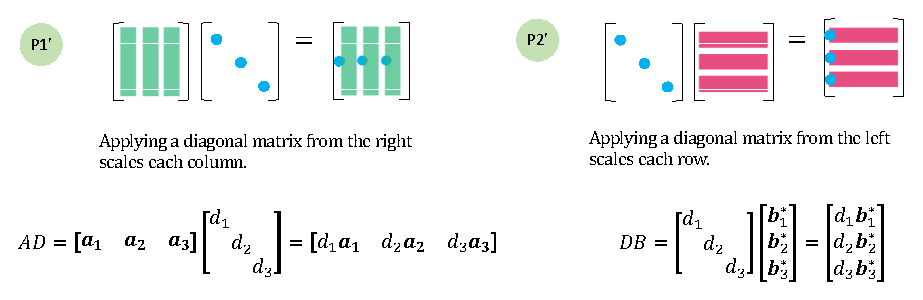
\includegraphics[scale=0.8]{Pattern11-22.eps}
  \caption{图 1$^\prime$, 2$^\prime$ - (P1$^\prime$), (P2$^\prime$)}
\end{figure}

(P1$^\prime$) 将对角线上的数乘以矩阵的列, 
而 (P2$^\prime$) 将对角线上的数乘以矩阵的行. 
两个分别为 (P1) 和 (P2) 的变体. 

\begin{figure}[H]
  \centering
  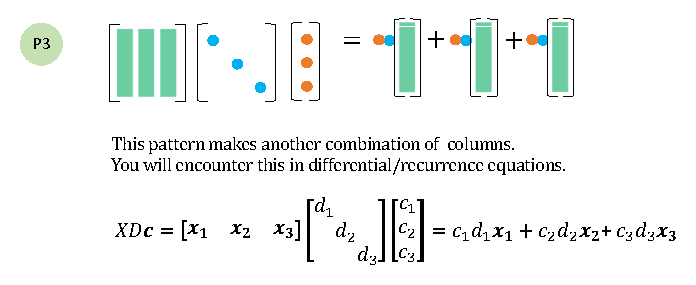
\includegraphics[scale=0.85]{Pattern3.eps}
  \caption{图 3 - (P3)}\label{fig:P3}
\end{figure}

当解决微分方程和递归方程时的也会出现这一模式: 

\begin{itemize}
  \item 6节 (p.201) Eigenvalues and Eigenvectors
  \item 6.4节 (p.243) Systems of Differential Equations
\end{itemize} 

\begin{align*}
  \frac{d \bm{u}(t) }{dt} &= A \bm{u}(t), \quad \bm{u}(0)=\bm{u}_0\\
  \bm{u}_{n+1} &= A \bm{u}_n, \quad \bm{u_0} = \bm{u}_0
\end{align*}

在两种问题中, 它的解都可以用$A$的特征值($\lambda_1, \lambda_2, \lambda_3$)、
特征向量$X=\begin{bmatrix} \bm{x}_1 & \bm{x}_2 & \bm{x}_3 \end{bmatrix}$
和系数$c=\begin{bmatrix} c_1 & c_2 & c_3 \end{bmatrix}\transp$表示. 
其中$C$是以$X$为基底的初始值$\bm{u}(0)=\bm{u}_0$的坐标.

\begin{equation*}
  \bm{u}_0 = c_1 \bm{x}_1 + c_2 \bm{x}_2 + c_3 \bm{x}_3
\end{equation*}
\begin{equation*}
  \bm{c} =
  \begin{bmatrix}
    c_1\\
    c_2\\
    c_3
  \end{bmatrix} = X^{-1} \bm{u}_0
\end{equation*}

以上两个问题的通解为: 

\begin{align*}
  \bm{u}(t) &= e^{At} \bm{u}_0 = X e^{\Lambda t} X^{-1} \bm{u_0} &= X e^{\Lambda t} \bm{c} &= c_1 e^{\lambda_1 t} \bm{x}_1 + c_2 e^{\lambda_2 t} \bm{x}_2 + c_3 e^{\lambda_3 t} \bm{x}_3\\
  \bm{u}_n &= A^n \bm{u}_0 = X \Lambda^n X^{-1} \bm{u_0} &= X \Lambda^n \bm{c} &= c_1 \lambda_1^n \bm{x}_1 + c_2 \lambda_2^n \bm{x}_2 + c_3 \lambda_3^n \bm{x}_3
\end{align*}

见Figure\ref{fig:P3}: 通过P3可以得到$XDc$. 

\begin{figure}[H]
  \centering
  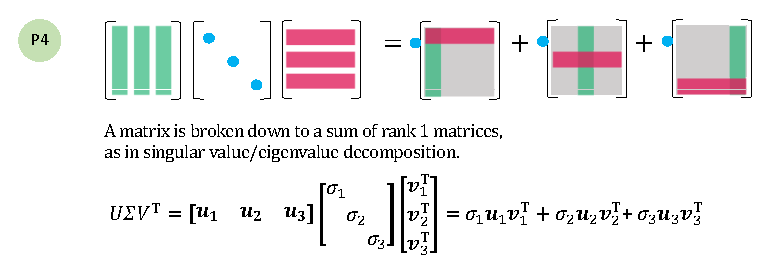
\includegraphics[scale=0.8]{Pattern4.eps}
  \caption{Pattern 4 - (P4)}
\end{figure}

P4在特征值分解和特异值分解中都会用到. 
两种分解都可以表示为三个矩阵之积, 其中中间的矩阵均为对角矩阵. 
且都可以表示为带特征值/特异值系数的秩1矩阵之积. 

更多细节将在下一节中讨论. 

\clearpage

\section{矩阵的五种分解}

\begin{itemize}
  \item 前言 p.vii, The Plan for the Book.
\end{itemize}
$A=CR, A=LU, A=QR, A=Q \Lambda Q\transp, A=U \Sigma V\transp$ 将一一说明.

\begin{table}[h]
  \begin{tabular}{lll}
    \Large{\boldmath $A=CR$} & 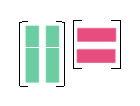
\includegraphics{A_CR.eps} &
    \begin{tabular}{l}
      $C$为$A$的线性无关列\\
      $R$为$A$的行阶梯形矩阵\\
      可推知 列秩 = 行秩
    \end{tabular}\\

    \Large{\boldmath $A=LU$} & 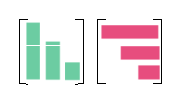
\includegraphics{A_LU.eps} &
    \begin{tabular}{l}
      $LU$分解通过\\
      高斯消去法\\
      (下三角)(上三角)
    \end{tabular}\\

    \Large{\boldmath $A=QR$} & 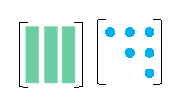
\includegraphics{A_QR.eps} &
    \begin{tabular}{l}
      $QR$分解为\\
      格拉姆-施密特正交化中的\\
      正交矩阵$Q$和三角矩阵$R$
    \end{tabular}\\
     
    \Large{\boldmath $S=Q\Lambda Q\transp$} & 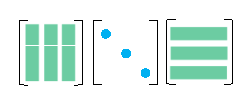
\includegraphics{A_QLQT.eps} &
    \begin{tabular}{l}
      对称矩阵$S$可以进行\\
      特征值分解\\
      特征向量组成$Q$, 特征值组成$\Lambda$
    \end{tabular}\\
  
    \Large{\boldmath $A=U\Sigma V\transp$} & 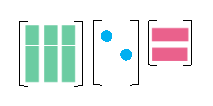
\includegraphics{A_USVT.eps} &
    \begin{tabular}{l}
      所有矩阵$A$的\\
      奇异值分解 \\
      奇异值组成$\Sigma$
    \end{tabular}
  \end{tabular}
  \caption{五种分解}

\end{table}

\subsection{$\boldsymbol{A=CR}$}

\begin{itemize}
  \item 1.4节 Matrix Multiplication and $\bm{A=CR}$ (p.29)
\end{itemize}

所有一般的长矩阵$A$都有相同的行秩和列秩. 
这个分解是理解这一定理最直观的方法. 
$C$由$A$的线性无关列组成, $R$为$A$的行阶梯形矩阵 (消除了零行).
$A=CR$将$A$化简为$r$的线性无关列$C$和线性无关行$R$的乘积. 

\begin{equation*}
  \begin{split}
    A &= CR\\
  \begin{bmatrix}
    1 & 2 & 3 \\
    2 & 3 & 5
  \end{bmatrix}
  & =
  \begin{bmatrix}
    1 & 2 \\
    2 & 3
  \end{bmatrix}
  \begin{bmatrix}
    1 & 0 & 1 \\
    0 & 1 & 1
  \end{bmatrix}
\end{split}
\end{equation*}

推导过程: 从左往右看$A$的列. 保留其中线性无关的列, 去掉可以由前者线性表出的列. 
则第1、2列被保留, 而第三列因为可以由前两列之和表示而被去掉. 
而要通过线性无关的1、2两列重新构造出$A$, 需要右乘一个行阶梯矩阵$R$. 

\begin{figure}[H]
  \centering
  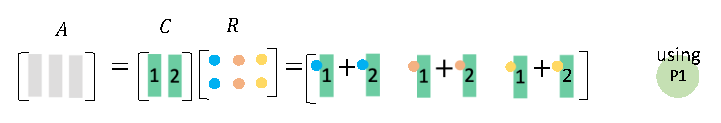
\includegraphics[scale=0.8]{CR1.eps}
  \caption{$CR$中列的秩}
\end{figure}

现在你会发现行的秩为2, 因为$C$中只有2个线性无关列. 
而$A$中所有的列都可以由$C$中的2列线性表出. 

\begin{figure}[H]
  \centering
  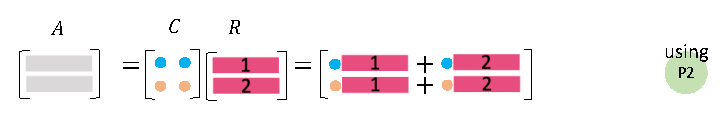
\includegraphics[scale=0.8]{CR2.eps}
  \caption{$CR$中行的秩}
\end{figure}

同样, 列秩也为2, 因为$R$中只有2个线性无关行, 且$A$中所有的行都可以由$R$中的2行线性表出. 

\subsection{$\boldsymbol{A=LU}$}

用高斯消除法求解$A\bm{x}=\bm{b}$也被称为$LU$分解. 
通常, 是$A$左乘一个初等行变换矩阵($E$)来得到一个上三角矩阵$U$. 

\begin{align*}
  EA &= U\\
  A &= E^{-1}U\\
\text{let} \; L = E^{-1}, \quad  A &= LU
\end{align*}

现在, 求解$A\bm{x}=\bm{b}$有2步: (1)求解$L\bm{c}=\bm{b}$, (2)代回$U\bm{x}=\bm{c}$. 


\begin{itemize}
  \item 2.3节 (p.57) Matrix Computations and $\bm{A=LU}$
\end{itemize}

在这里, 我们直接通过$A$计算$L$和$U$.

\begin{equation*}
  A = 
      \begin{bmatrix}
        |\\
        \bm{l}_1\\
        |
      \end{bmatrix}
      \begin{bmatrix}
        -  \bm{u}^*_1  -
      \end{bmatrix}
  +  \begin{bmatrix}
      0 & \begin{matrix} 0 & 0 \end{matrix}\\
      \begin{matrix} 0 \\ 0 \end{matrix} & A_2
    \end{bmatrix}
  = 
  \begin{bmatrix}
    |\\
    \bm{l}_1\\
    |
  \end{bmatrix}
  \begin{bmatrix}
    - \bm{u}^*_1 -
  \end{bmatrix}
  +
  \begin{bmatrix}
    |\\
    \bm{l}_2\\
    |
  \end{bmatrix}
  \begin{bmatrix}
    - \bm{u}^*_2  -
  \end{bmatrix}
  +  \begin{bmatrix}
  0 & 0 & 0\\
  0 & 0 & 0 \\
  0 & 0 & A_3
  \end{bmatrix} = LU
\end{equation*}
 

\begin{figure}[H]
  \centering
  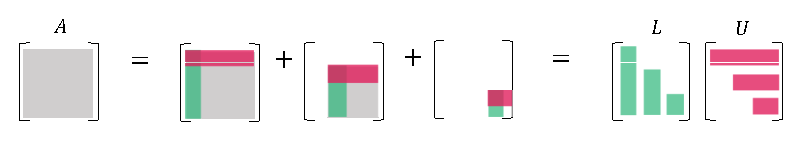
\includegraphics[scale=0.8]{LU1.eps}
\caption{$A的递归秩1矩阵分离$}
\end{figure}

要计算$L$和$U$, 首先分离出由$A$的第一行和第一列组成的外积. 
余下的部分为$A_2$. 
递归执行此操作, 将$A$分解为秩1矩阵之和. 


\begin{figure}[H]
  \centering
  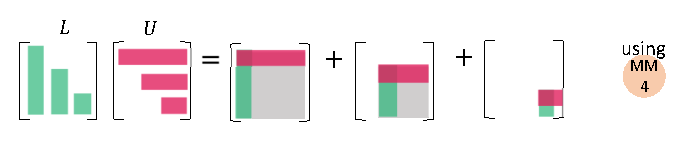
\includegraphics[scale=0.8]{LU2.eps}
\caption{由$LU$重新构造$A$}
\end{figure}

由$L$乘以$U$来重新构造$A$则相对简单. 

\subsection{$\boldsymbol{A=QR}$}

$A=QR$是在保持$\bm{C}(A) = \bm{C}(Q)$的条件下, 将$A$转化为正交矩阵$Q$.

\begin{itemize}
  \item 4.4节 Orthogonal matrices and Gram-Schmidt (p.165)
\end{itemize}

在格拉姆-施密特正交化中, 首先, 单位化的$\bm{a}_1$被用作$\bm{q}_1$, 
然后求出$\bm{a}_2$与$\bm{q}_1$正交所得到的$\bm{q}_2$, 以此类推. 

\begin{align*}
  \bm{q}_1 &= \bm{a}_1/||\bm{a}_1|| \\
  \bm{q}_2 &= \bm{a}_2 - (\bm{q}_1\transp \bm{a}_2)\bm{q}_1 , \quad \bm{q}_2 = \bm{q}_2/||\bm{q}_2|| \\
  \bm{q}_3 &= \bm{a}_3 - (\bm{q}_1\transp \bm{a}_3)\bm{q}_1 - (\bm{q}_2\transp \bm{a}_3)\bm{q}_2, \quad \bm{q}_3 = \bm{q}_3/||\bm{q}_3||
\end{align*}

或者你也可以写作$r_{ij} = \bm{q}_i\transp \bm{a}_j$:

\begin{align*}
  \bm{a}_1 &= r_{11}\bm{q}_1\\
  \bm{a}_2 &= r_{12}\bm{q}_1 + r_{22} \bm{q}_2\\
  \bm{a}_3 &= r_{13}\bm{q}_1 + r_{23} \bm{q}_2 + r_{33} \bm{q}_3
\end{align*}

原本的$A$就可以表示为$QR$: 正交矩阵乘以上三角矩阵. 

\begin{gather*}
  A = 
  \begin{bmatrix}
    | & | & |\\
    \bm{q}_1 & \bm{q}_2 & \bm{q}_3\\
    | & | & |
  \end{bmatrix}
  \begin{bmatrix}
    r_{11} & r_{12} & r_{13}\\
           & r_{22} & r_{23}\\
           &        & r_{33}
  \end{bmatrix} = QR\\
  \\
  Q Q\transp=Q\transp Q = I
\end{gather*}

\begin{figure}[H]
  \centering
  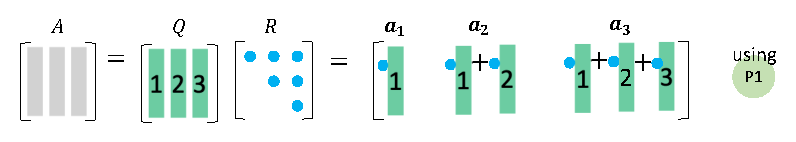
\includegraphics[scale=0.8]{QR.eps}
  \caption{$A=QR$}
\end{figure}

$A$的列向量就可以转化为一个正交集合: $Q$的列向量. 
$A$的每一个列向量都可以用$Q$和上三角矩阵$R$重新构造出. 

图释可以回头看P1.


\subsection{$\boldsymbol{S=Q \Lambda Q\transp}$}

所有对称矩阵$S$都必须有实特征值和正交特征向量. 
特征值是$\Lambda$的对角元素, 特征向量在$Q$中. 

\begin{itemize}
  \item 6.3节 (p.227) Symmetric Positive Definite Matrices
\end{itemize}

\begin{align*}
  S = Q \Lambda Q\transp
&= \begin{bmatrix}
    | & | & |\\
    \bm{q}_1 & \bm{q}_2 & \bm{q}_3\\
    | & | & |
  \end{bmatrix}
  \begin{bmatrix}
    \lambda_1 \\
           & \lambda_2 & \\
           & & \lambda_3
  \end{bmatrix}
  \begin{bmatrix}
  - \bm{q}_1\transp -\\
  - \bm{q}_2\transp -\\
  - \bm{q}_3\transp -
  \end{bmatrix}\\
  \\
  &=
  \lambda_1 \begin{bmatrix}
    |\\
    \bm{q}_1\\
    |
  \end{bmatrix}
  \begin{bmatrix}
    - \bm{q}_1\transp - 
  \end{bmatrix}
  +
  \lambda_2 \begin{bmatrix}
  |\\
  \bm{q}_2\\
  |
  \end{bmatrix}
  \begin{bmatrix}
  - \bm{q}_2\transp -
  \end{bmatrix} 
  +
  \lambda_3 \begin{bmatrix}
    |\\
    \bm{q}_3 \\
    |
  \end{bmatrix}
  \begin{bmatrix}
    - \bm{q}_3\transp -
  \end{bmatrix} \\
&= \lambda_1 P_1 + \lambda_2 P_2 + \lambda_3 P_3
\end{align*}

\begin{equation*}
  P_1=\bm{q}_1 \bm{q}_1\transp, \quad P_2=\bm{q}_2 \bm{q}_2\transp, \quad P_3=\bm{q}_3 \bm{q}_3\transp
\end{equation*}


\begin{figure}[H]
  \centering
  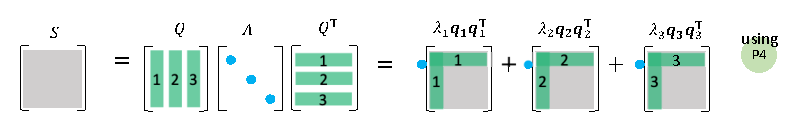
\includegraphics[scale=0.8]{EVD.eps}
  \caption{$S=Q \Lambda Q\transp$}
\end{figure}

一个对乘矩阵$S$通过一个正交矩阵$Q$和它的转置矩阵, 对角化为$\Lambda$. 
然后被分解为一阶投影矩阵$P=qq\transp$的组合. 这就是谱定理. 

注意, 这里的分解用到了P4.

\begin{gather*}
  S=S\transp = \lambda_1 P_1 + \lambda_2 P_2 + \lambda_3 P_3\\
  QQ\transp = P_1 + P_2 + P_3 = I \\
  P_1 P_2 = P_2 P_3 = P_3 P_1 = O\\
  P_1^2 =P_1=P_1\transp, \quad P_2^2=P_2=P_2\transp, \quad P_3^2=P_3=P_3\transp
\end{gather*}

\subsection{$\boldsymbol{A=U \Sigma V\transp}$}


\begin{itemize}
  \item 7.1节 (p.259) Singular Values and Singular Vecrtors
\end{itemize}

包括长方阵在内的所有矩阵都具有奇异值分解(SVD). 
$A=U \Sigma V\transp$中, 有$A$的奇异向量$U$和$V$. 
奇异值则排列在$\Sigma$的对角线上. 
下图就是“简化版”的SVD. 


\begin{figure}[H]
  \centering
  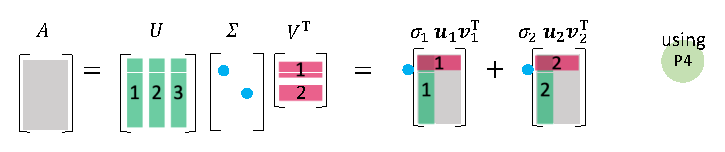
\includegraphics[scale=0.8]{SVD.eps}
  \caption{$A=U \Sigma V\transp$}
\end{figure}

你可以发现, $V$是$\mathbb{R}^n$ ($A\transp A$的特征向量) 的标准正交基, 
而$U$是 $\mathbb{R}^m$ ($AA\transp$的特征向量) 的标准正交基. 
它们共同将$A$对角化为$\Sigma$. 
这也可以表示为秩1矩阵的线性组合. 

\begin{align*}
  A = U \Sigma V\transp =
  \begin{bmatrix}
    | & | & |\\
    \bm{u}_1 & \bm{u}_2 & \bm{u}_3\\
    | & | & |
  \end{bmatrix}
  \begin{bmatrix}
    \sigma_1 \\
           & \sigma_2 \\
           & &
  \end{bmatrix}
  \begin{bmatrix}
  - \bm{v}_1\transp -\\
  - \bm{v}_2\transp -
  \end{bmatrix}
  & =
  \sigma_1 \begin{bmatrix}
    |\\
    \bm{u}_1\\
    |
  \end{bmatrix}
  \begin{bmatrix}
    - \bm{v}_1\transp - 
  \end{bmatrix}
  +
  \sigma_2 \begin{bmatrix}
  |\\
  \bm{u}_2\\
  |
  \end{bmatrix}
  \begin{bmatrix}
  - \bm{v}_2\transp -
  \end{bmatrix} \\
& = \sigma_1 \bm{u}_1 \bm{v}_1\transp + \sigma_2 \bm{u}_2 \bm{v}_2\transp
\end{align*}

注意: 

\begin{align*}
  U U\transp &= I_m \\
  V V\transp &= I_n
\end{align*}

图释见P4.

\section*{总结和致谢}

我展示了矩阵/向量乘法的系统可视化与它们在五种矩阵分解中的应用. 
我希望你能够喜欢它们、通过它们加深对线性代数的理解. 

Ashley Fernandes 在排版时帮我美化了这篇论文, 使它更加一致和专业. 

在结束这篇论文之前, 我要感谢 Gilbert Strang 教授出版了《Linear Algebra for Everyone》一书. 
它引导我们通过新的视角去了解线性代数中这些美丽的风景. 
其中介绍了当代和传统的数据科学和机器学习, 每个人都可以通过实用的方式对它的基本思想进行基本理解. 矩阵世界的重要组成部分. 

\section*{参考文献与相关工作}
\begin{enumerate}
  \item 
  Gilbert Strang(2020),\emph{Linear Algebra for Everyone}, Wellesley Cambridge Press.,\\
  \href{http://math.mit.edu/everyone}{http://math.mit.edu/everyone}
  \item
  Gilbert Strang(2016), \emph{Introduction to Linear Algebra},Wellesley Cambridge Press, 5th ed.,\\
  \href{http://math.mit.edu/linearalgebra}{http://math.mit.edu/linearalgebra}
  \item Kenji Hiranabe(2021), \emph{Map of Eigenvalues}, An Agile Way(blog),\\
  \href{https://anagileway.com/2021/10/01/map-of-eigenvalues/}{https://anagileway.com/2021/10/01/map-of-eigenvalues/}\\
  \begin{figure}[H]
    \centering
    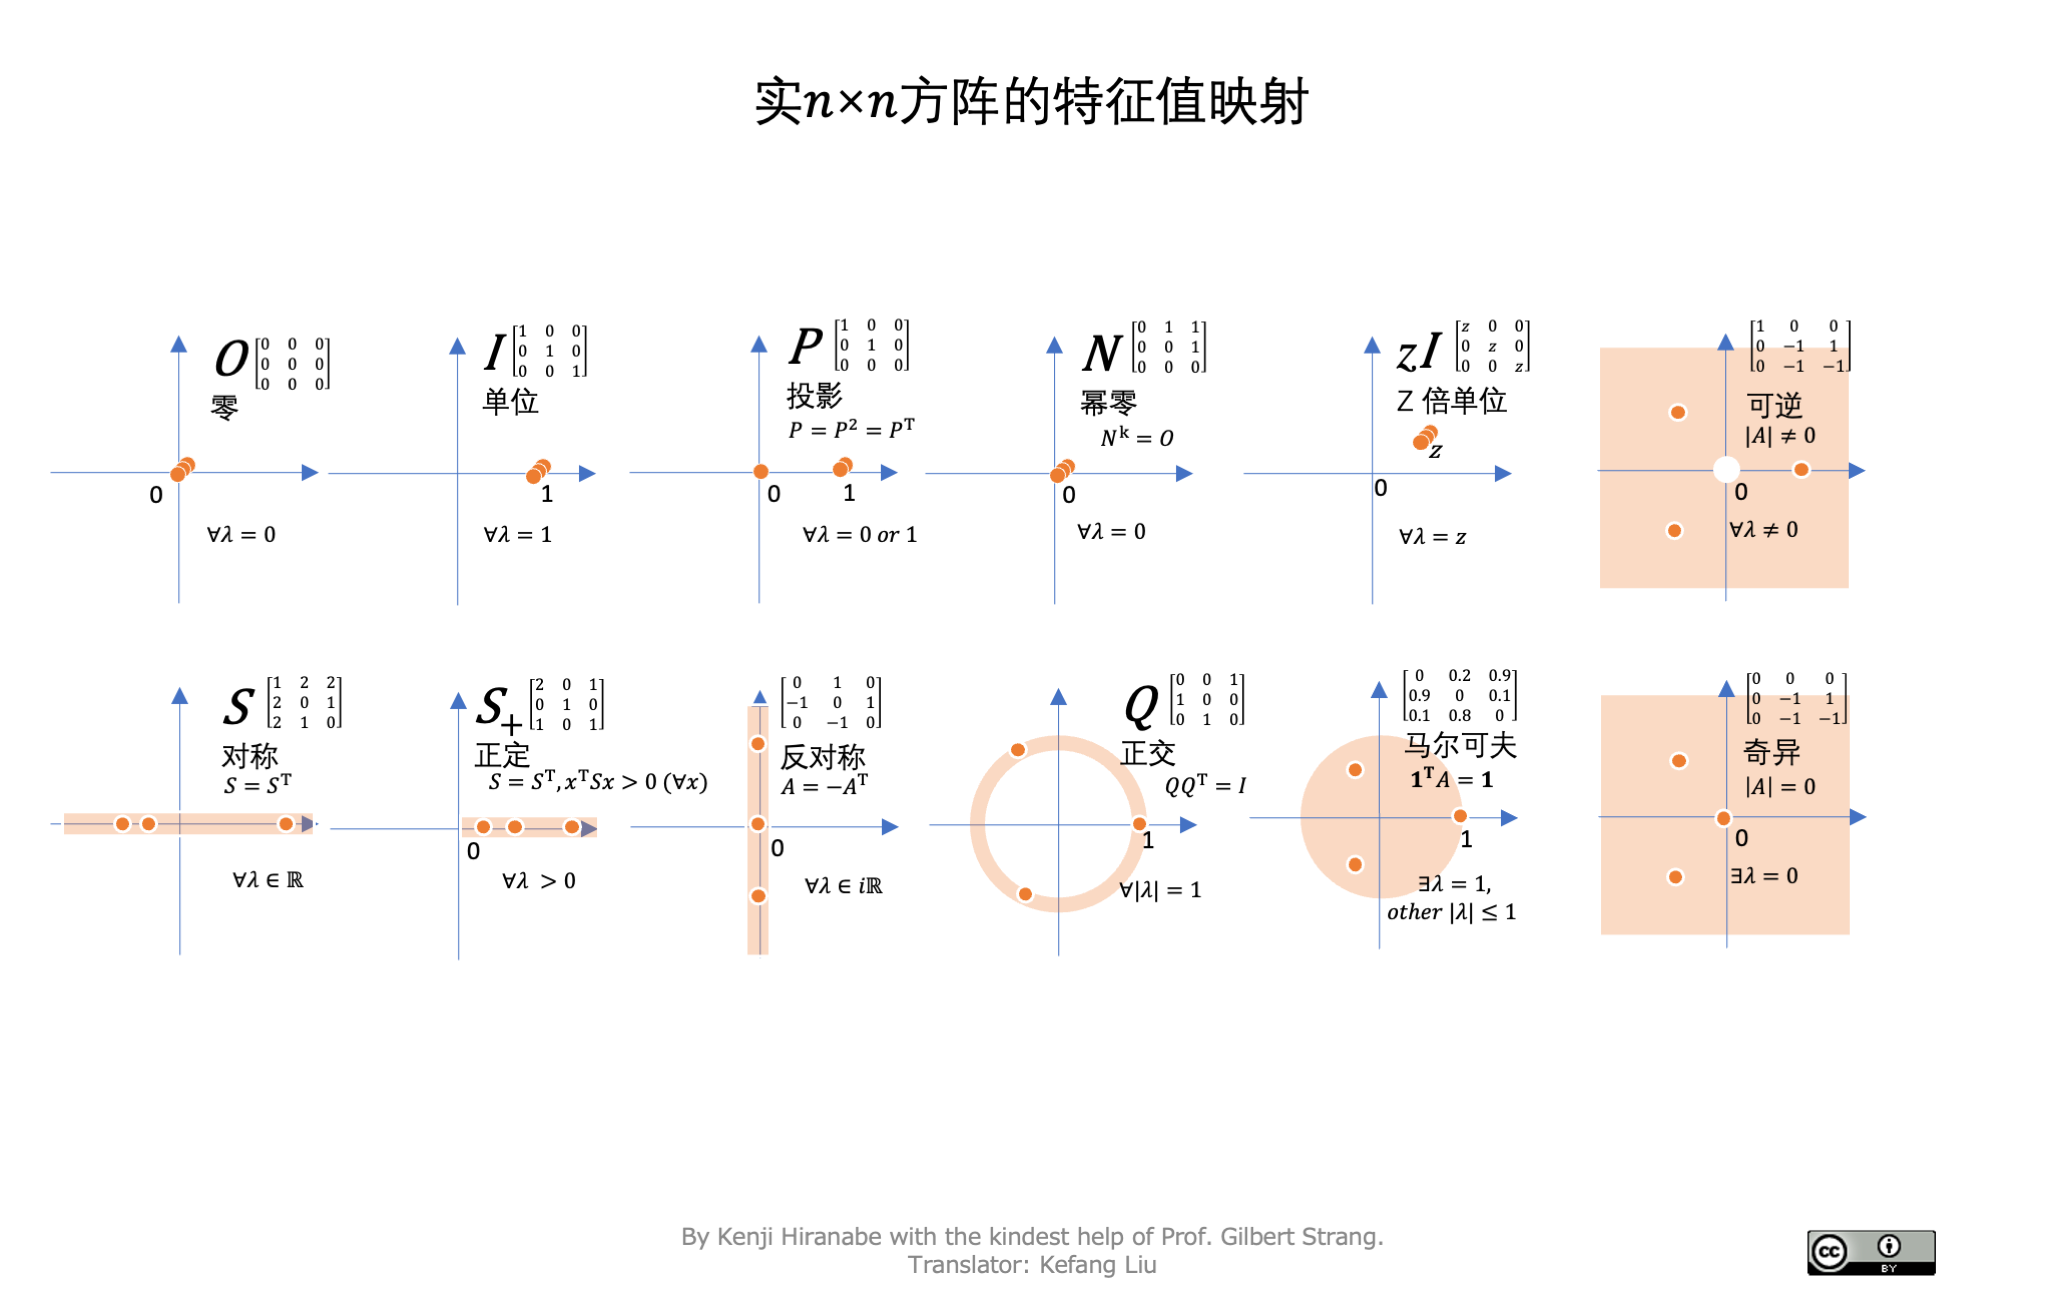
\includegraphics[keepaspectratio, width=\linewidth]{MapofEigenvalues-zh-CN.png}
    \caption{特征值图}
  \end{figure}
  \item Kenji Hiranabe(2020), \emph{Matrix World}, An Agile Way(blog),\\
  \href{https://anagileway.com/2020/09/29/matrix-world-in-linear-algebra-for-everyone/}{https://anagileway.com/2020/09/29/matrix-world-in-linear-algebra-for-everyone/}
  \begin{figure}[H]
    \centering
    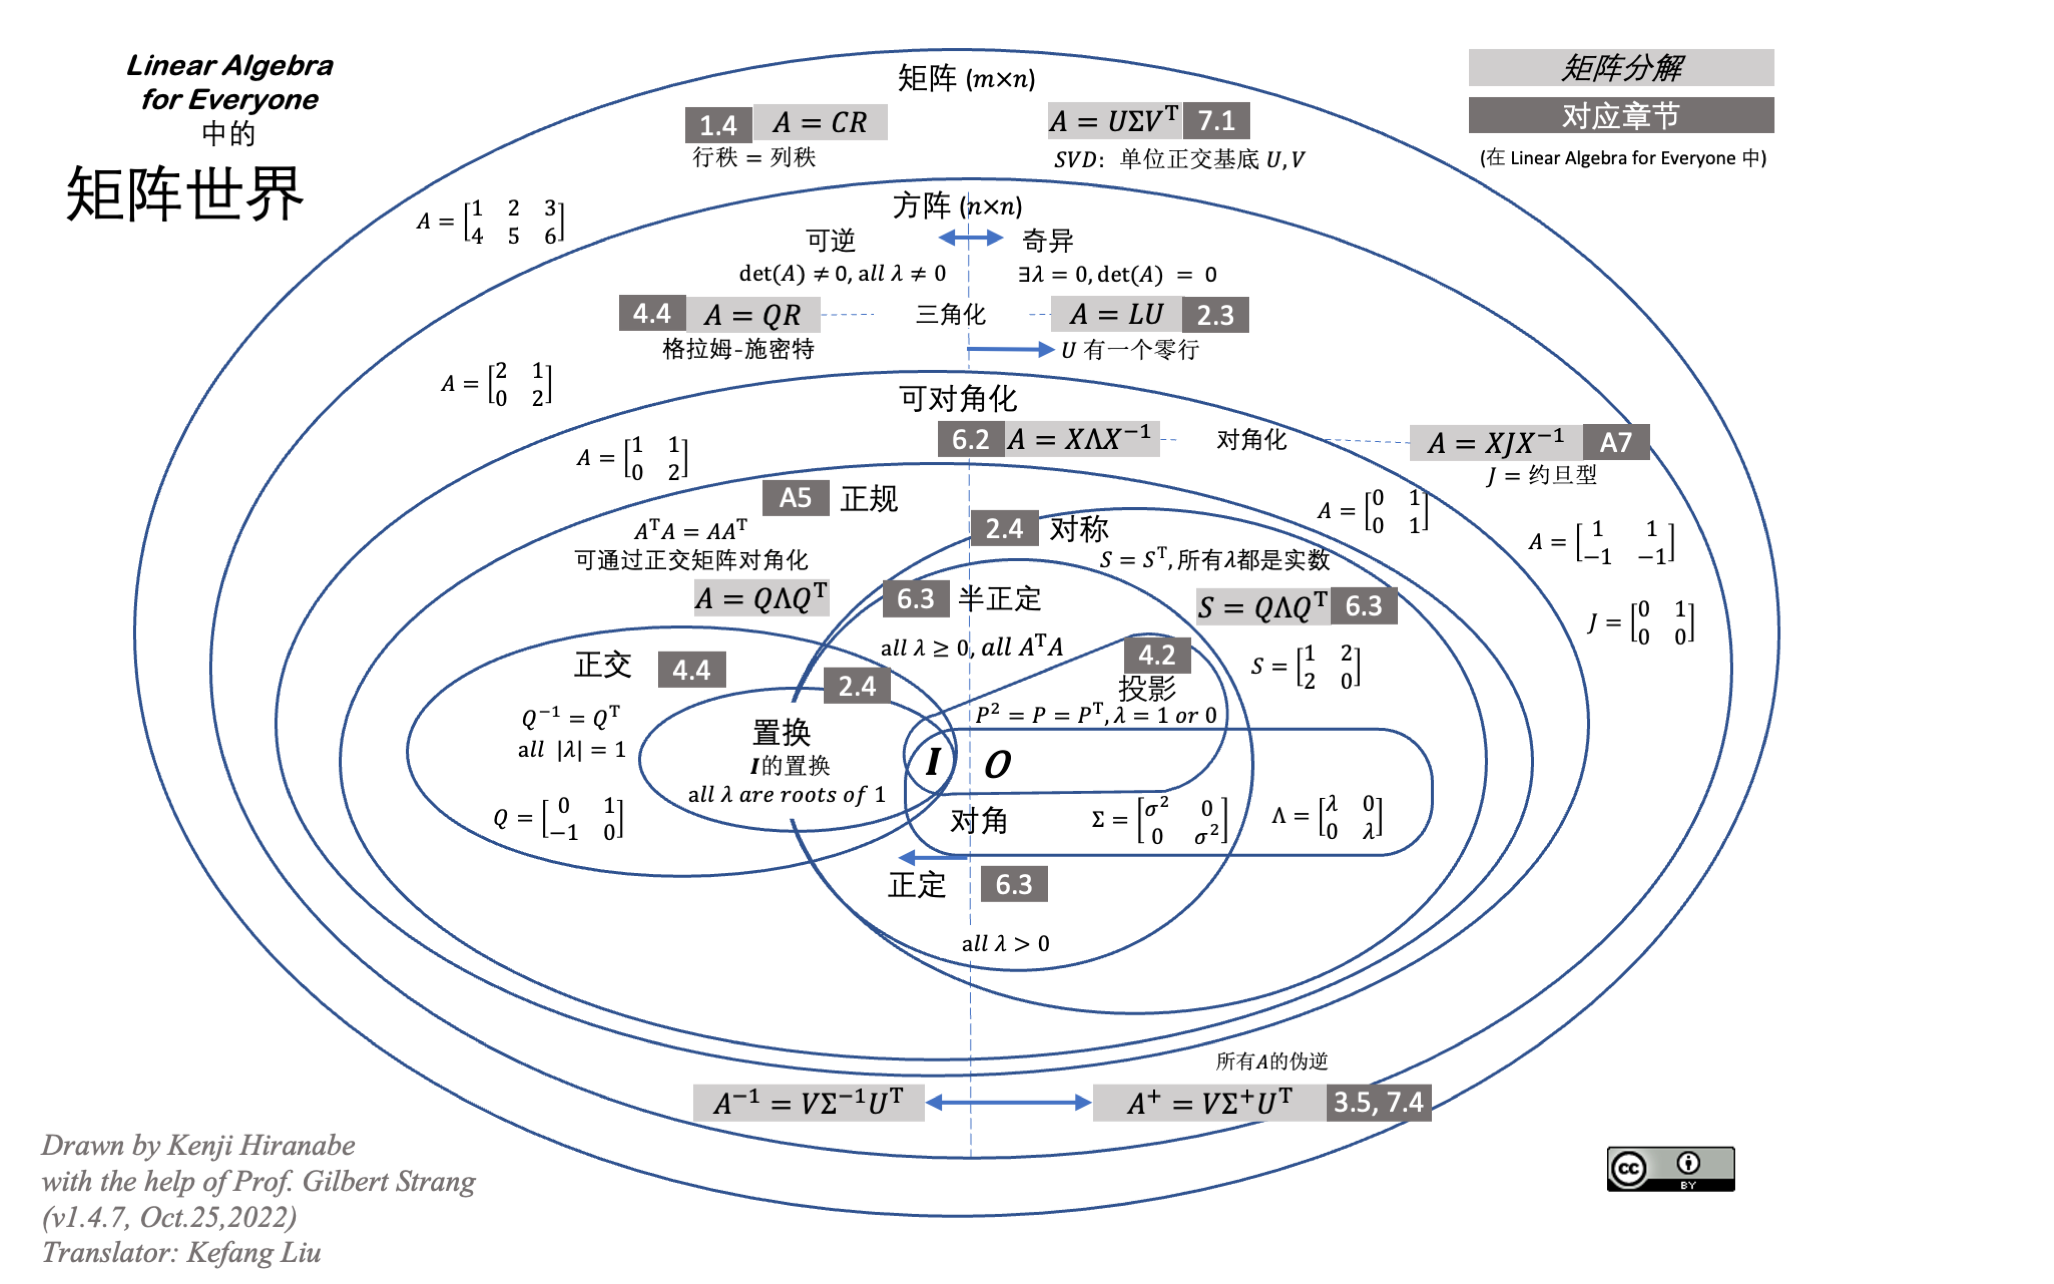
\includegraphics[keepaspectratio, width=\linewidth]{MatrixWorld-zh-CN.png}
    \caption{矩阵世界}
  \end{figure}
\end{enumerate}

\end{document}